We have developed a plugin which stores data in a format which enables performing semantic analysis on the data and uses PLFS for high I/O throughput. 
Instead of storing all objects in a single file, it stores every HDF5 object in a separate location, so that data from different objects is not contained in the same file. In short, we provide a raw mapping of HDF5 objects to the file system. 
HDF5 files and groups are stored as directories, whereas datasets and attributes, which contain raw data, are stored in files created using PLFS. 
Consider the example shown in figure~\ref{hdf5_example}. Using the plugin, file Sample.h5 is stored as a directory. Group G1 is stored as a directory under it, and datasets D1 and D2 are files. Attribute A1 is a file created at the same location as dataset D1 to which it is attached. Additionally, the name of the attribute is stored as \textit{dataset name}.\textit{attribute name} to denote the dataset to which the attribute is attached. Thus these objects are stored at the following paths:\\
/Sample.h5/\\
/Sample.h5/G1\\
/Sample.h5/G1/D3\\
/Sample.h5/D1\\
/Sample.h5/D1.A1\\
/Sample.h5/D2\\

We can see that the relationship between the objects is represented by their relative paths at the file system. That is, the path /Sample.h5/G1/D3 tells us that D3 is a dataset belonging to Group G1 under the root group of the file. This approach gives us the ability to distinguish HDF5 objects inside the storage system. Also, the plugin eliminates the need to explicitly store the metadata describing the relationship between objects. Metadata about datasets, such as the datatype, extent, dimensions etc. are stored as Xattrs. 
 
%\begin{figure}[!t]
%\centering
%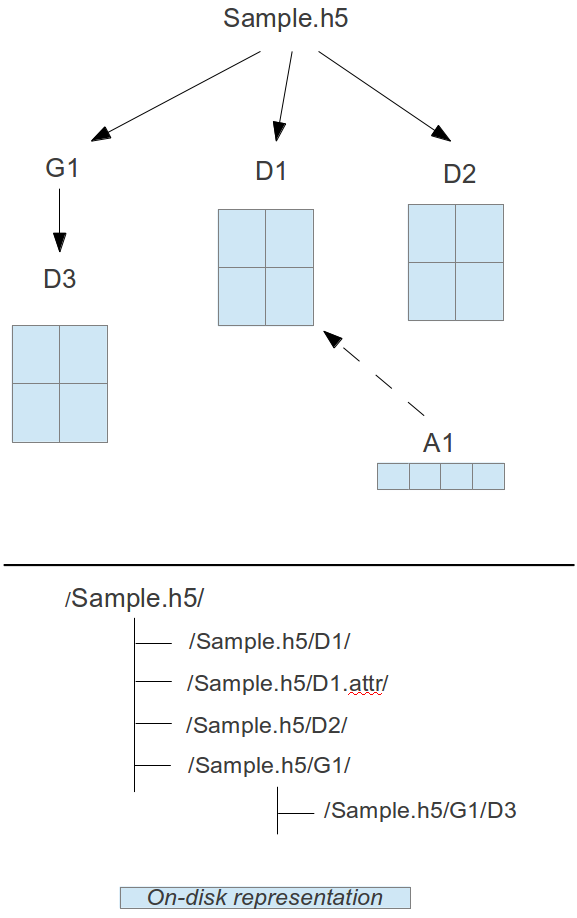
\includegraphics[width=2.5in]{hdf5_example_plugin}
%\caption{HDF5 file created using our PLFS plugin}
%\label{hdf5_example_plugin}
%\end{figure}


Our plugin makes direct calls to the PLFS API. For the current version, we do not support collective I/O operations. It should be noted that HDF5 when used natively with MPI-IO allows users to specify whether collective I/O should be used for reading and writing data. 

The above format of storing data allows us to perform at least two different analysis optimizations.  To illustrate via an example, imagine storing a three-dimensional ocean model within a PLFS file. The storage system sees the file as an opaque linear array of bytes.  With the structure, however, PLFS can provide \textit{active analysis} as well as \textit{semantic restructuring}.  

Active analysis borrows the transducers idea from the Semantic File System~\cite{semantic_fs} which has since been productized in Google's BigTable and Apache Hbase technologies~\cite{google_coprocessors,GFS,apache_hbase}.  With active analysis, the application can ship a data parser function when it creates the PLFS file.  As the data is written into PLFS, PLFS can apply the data function on the streaming data.  The function will output key-value pairs which PLFS can embed in its extensible metadata.  In this example, one simple function might record the height of the largest wave.  Due to PLFS's model of storing a logical file across multiple physical files, the PLFS extensible metadata can record the height of the largest wave within each physical file.  However, given that PLFS now understands the structure of the logical file, these multiple physical files, within the PLFS container, are more accurately thought of as shards.  In a future burst buffer architecture~\cite{burst_buffers}, these semantic shards will be spread across multiple burst buffer nodes.  Therefore, subsequent analysis of the ocean model can quickly find the burst buffer containing the shard with the largest wave by searching a small amount of extensible metadata instead of scanning the entire ocean model.

Semantic restructuring is the idea of reorganizing the data into a new set of semantic shards.  This would be done to speed future analysis routines.  For example, assume that the ocean model was originally sharded using a row-order organization (i.e. across latitude instead of longitude).  An analysis routine which will explore the model along a column-ordering will suffer poor performance with the row-order organization as its access pattern will result in a large number of small reads from a large set of semantic shards.  However, by knowing the semantic structure, the analysis routine can request a semantic restructuring which will be a compact, intuitively described request such as "restructure into row-ordering."  Without structural knowledge, a semantic restructuring would be significantly more complicated: the analysis routine would have to send a large list of logical offsets to PLFS to inform it of expected read patterns.  In an exascale system, the list of logical offsets will be in the order of one billion.  Semantic restructuring shrinks the size of the request to a small constant value.

%The following table lists the VOL functions currently provided by the PLFS plugin:
%\begin{itemize}
%\item Attribute yes
%\item Dataset yes
%\item File yes
%\item Group yes
%\item Object No
%\item Link No
%\end{itemize}

